\documentclass[11pt]{article}

% ---------------------------------------------------
% Packages
% ---------------------------------------------------
\usepackage[margin=1in]{geometry}
\usepackage{tikz}
\usepackage{xcolor}
\usepackage{helvet}
\usepackage{enumitem}
\usepackage{titlesec}
\renewcommand{\familydefault}{\sfdefault}

\usetikzlibrary{arrows.meta,positioning,fit,calc,backgrounds}

% ---------------------------------------------------
% Brand Colors
% ---------------------------------------------------
\definecolor{brandNavy}{HTML}{0B1220}
\definecolor{brandTeal}{HTML}{06B6D4}
\definecolor{brandGreen}{HTML}{2E7D32}
\definecolor{brandGrayLight}{HTML}{F3F4F6}
\definecolor{brandGray}{HTML}{E5E7EB}

% ---------------------------------------------------
% Layout + Headings
% ---------------------------------------------------
\setlength{\parskip}{6pt}
\setlength{\parindent}{0pt}

\titleformat{\section}{\large\bfseries\color{brandNavy}}{}{0pt}{}
\titlespacing{\section}{0pt}{14pt}{6pt}

\titleformat{\subsection}{\bfseries\color{brandNavy}}{}{0pt}{}
\titlespacing{\subsection}{0pt}{10pt}{4pt}

% ---------------------------------------------------
\begin{document}

{\Huge\bfseries GreenieRE \& Reinsurance Analytics}\\[2pt]
{\Large\bfseries Phase 1 Technical Architecture}\\[4pt]
{\small MGA Bordereaux Automation, LIDAC Eligibility, and ZIP Accumulation Risk}

\vspace{0.8em}
\hrule height 1pt
\vspace{1em}

% ============================================================
\section{Objectives}

Phase~1 delivers an end–to–end data pipeline that turns raw carrier and MGA
bordereaux into:

\begin{itemize}[leftmargin=1.6em,itemsep=3pt]
  \item \textbf{Clean, standardized project records} across multiple carriers.
  \item \textbf{ZIP and census–tract level intelligence} using HUD crosswalks.
  \item \textbf{LIDAC / CEJST-style eligibility tags} at the tract level.
  \item \textbf{Intacct-ready journal entries} for premiums, commissions, and fees.
  \item \textbf{ZIP-level accumulation flags} to highlight clustering of exposure
        across carriers.
  \item \textbf{Clear export files} that Wenhua can inspect, audit, and load into
        existing systems.
\end{itemize}

The design is intentionally simple: one repeatable pipeline that can run for any
MGA or carrier that supplies a bordereaux file with the current column structure.

% ============================================================
\section{System Architecture Diagram (Phase 1)}

\begin{figure}[htpb]
\centering
\resizebox{0.85\textwidth}{!}{
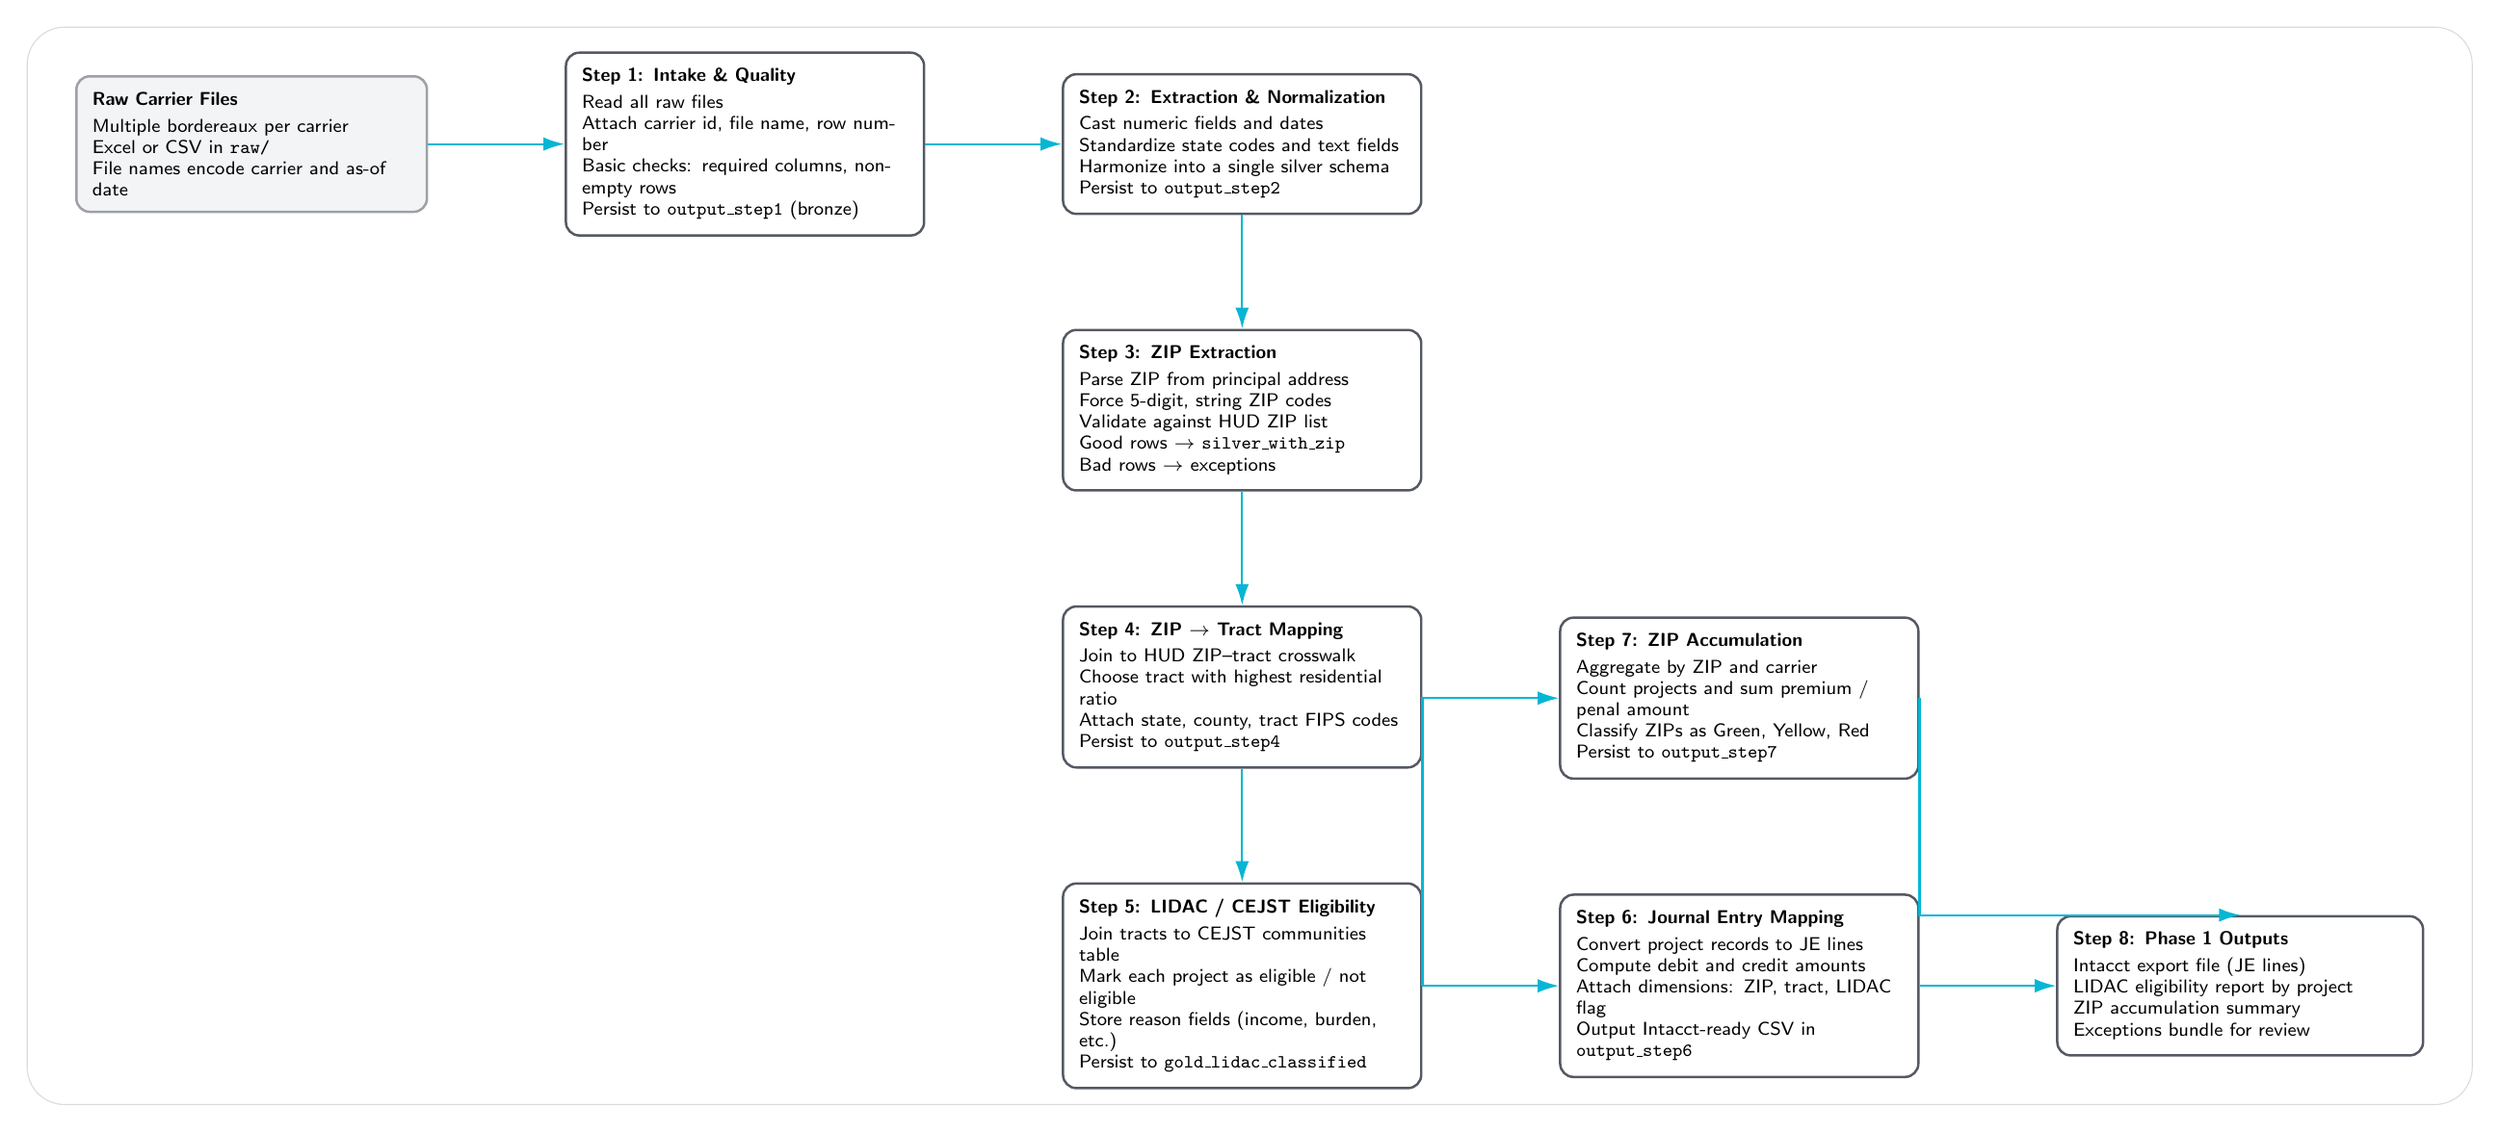
\begin{tikzpicture}[
    font=\scriptsize,
    node distance=1.7cm and 1.7cm,
    process/.style={
        rectangle,
        rounded corners=5pt,
        draw=brandNavy!70,
        line width=0.9pt,
        fill=white,
        text width=4.3cm,
        inner sep=6pt,
        align=left
    },
    datastore/.style={
        rectangle,
        rounded corners=5pt,
        draw=brandNavy!40,
        line width=0.9pt,
        fill=brandGrayLight,
        text width=4.2cm,
        inner sep=6pt,
        align=left
    },
    outputbox/.style={
        rectangle,
        rounded corners=5pt,
        draw=brandNavy!70,
        line width=0.9pt,
        fill=white,
        text width=4.4cm,
        inner sep=6pt,
        align=left
    },
    flow/.style={
        -{Latex[length=2.8mm,width=1.8mm]},
        thick,
        draw=brandTeal
    }
]

% -------------------- Left: Raw Data -------------------------
\node[datastore] (raw) {
  \textbf{Raw Carrier Files}\\[2pt]
  Multiple bordereaux per carrier\\
  Excel or CSV in \texttt{raw/}\\
  File names encode carrier and as-of date
};

% -------------------- Processing Steps -----------------------
\node[process, right=1.8cm of raw] (step1) {
  \textbf{Step 1: Intake \& Quality}\\[2pt]
  Read all raw files\\
  Attach carrier id, file name, row number\\
  Basic checks: required columns, non-empty rows\\
  Persist to \texttt{output\_step1} (bronze)
};

\node[process, right=1.8cm of step1] (step2) {
  \textbf{Step 2: Extraction \& Normalization}\\[2pt]
  Cast numeric fields and dates\\
  Standardize state codes and text fields\\
  Harmonize into a single silver schema\\
  Persist to \texttt{output\_step2}
};

\node[process, below=1.5cm of step2] (step3) {
  \textbf{Step 3: ZIP Extraction}\\[2pt]
  Parse ZIP from principal address\\
  Force 5-digit, string ZIP codes\\
  Validate against HUD ZIP list\\
  Good rows $\rightarrow$ \texttt{silver\_with\_zip}\\
  Bad rows $\rightarrow$ exceptions
};

\node[process, below=1.5cm of step3] (step4) {
  \textbf{Step 4: ZIP $\rightarrow$ Tract Mapping}\\[2pt]
  Join to HUD ZIP--tract crosswalk\\
  Choose tract with highest residential ratio\\
  Attach state, county, tract FIPS codes\\
  Persist to \texttt{output\_step4}
};

\node[process, below=1.5cm of step4] (step5) {
  \textbf{Step 5: LIDAC / CEJST Eligibility}\\[2pt]
  Join tracts to CEJST communities table\\
  Mark each project as eligible / not eligible\\
  Store reason fields (income, burden, etc.)\\
  Persist to \texttt{gold\_lidac\_classified}
};

\node[process, right=1.8cm of step5] (step6) {
  \textbf{Step 6: Journal Entry Mapping}\\[2pt]
  Convert project records to JE lines\\
  Compute debit and credit amounts\\
  Attach dimensions: ZIP, tract, LIDAC flag\\
  Output Intacct-ready CSV in \texttt{output\_step6}
};

\node[process, above=1.5cm of step6] (step7) {
  \textbf{Step 7: ZIP Accumulation}\\[2pt]
  Aggregate by ZIP and carrier\\
  Count projects and sum premium / penal amount\\
  Classify ZIPs as Green, Yellow, Red\\
  Persist to \texttt{output\_step7}
};

% -------------------- Outputs -------------------------------
\node[outputbox, right=1.8cm of step6] (outputs) {
  \textbf{Step 8: Phase 1 Outputs}\\[2pt]
  Intacct export file (JE lines)\\
  LIDAC eligibility report by project\\
  ZIP accumulation summary\\
  Exceptions bundle for review
};

% -------------------- Flows ---------------------------------
\draw[flow] (raw.east) -- (step1.west);
\draw[flow] (step1.east) -- (step2.west);
\draw[flow] (step2.south) -- (step3.north);
\draw[flow] (step3.south) -- (step4.north);
\draw[flow] (step4.south) -- (step5.north);
\draw[flow] (step5.east) -- (step6.west);
\draw[flow] (step5.east) |- (step7.west);
\draw[flow] (step6.east) -- (outputs.west);
\draw[flow] (step7.east) |- (outputs.north);

% Soft bounding box
\begin{scope}[on background layer]
\node[
  draw=brandNavy!15,
  rounded corners=14pt,
  inner sep=18pt,
  fit=(raw) (outputs)
] {};
\end{scope}

\end{tikzpicture}}
\caption{Phase 1 end-to-end pipeline from raw bordereaux files to accounting and risk outputs.}
\end{figure}

\clearpage

% ============================================================
\section{Pipeline Steps (Business-Facing Description)}

\subsection*{Step 1 \;--\; Intake and Data Quality (Bronze Layer)}

\textbf{What runs.} The \texttt{step1\_intake\_and\_quality.py} script scans the
\texttt{raw/} folder, reads every carrier file (CSV or Excel), and appends:

\begin{itemize}[leftmargin=1.6em,itemsep=2pt]
  \item Carrier identifier (parsed from file name, e.g.\ C001, C002, C003).
  \item Source file name and row number for full lineage.
  \item Ingestion timestamp in UTC.
\end{itemize}

\textbf{Why it matters.}  
This establishes a single, auditable ``bronze'' table where every bordereaux row
can be traced back to the original file and line. If a number looks wrong later,
we can immediately see which carrier file it came from.

\subsection*{Step 2 \;--\; Extraction and Normalization (Silver Layer)}

\textbf{What runs.} The \texttt{step2\_extraction\_normalization.py} script:

\begin{itemize}[leftmargin=1.6em,itemsep=2pt]
  \item Casts numeric columns (\emph{Gross Premium}, \emph{Net Premium},
        \emph{Commission}, \emph{Penal Amount}) into clean decimals.
  \item Converts dates (\emph{Effective}, \emph{Expiration}, \emph{As-of Date})
        into ISO date format.
  \item Normalizes state codes (e.g.\ “Pa” and “PA” both become “PA”).
  \item Trims whitespace, cleans text, and applies a consistent column schema
        defined in \texttt{schema\_registry.py}.
\end{itemize}

\textbf{Why it matters.}  
The result is a single, standardized ``silver'' table across all carriers, ready
for geo-joining, eligibility tagging, and accounting logic.

\subsection*{Step 3 \;--\; ZIP Extraction and Validation}

\textbf{What runs.} The \texttt{step3\_zip\_extraction.py} script:

\begin{itemize}[leftmargin=1.6em,itemsep=2pt]
  \item Parses the ZIP code out of the \emph{Principal / Account Mailing Address}.
  \item Ensures the ZIP is always stored as a 5-character string
        (e.g.\ ``02115'', not ``2115'').
  \item Validates the ZIP against the HUD ZIP list and marks:
        \emph{zip\_valid\_flag} and \emph{zip\_error\_reason}.
  \item Routes invalid or missing ZIPs into an exceptions file.
\end{itemize}

\textbf{Why it matters.}  
Clean and validated ZIP codes are the foundation for all tract-level and LIDAC
calculations. Fixing them here prevents downstream errors.

\subsection*{Step 4 \;--\; ZIP to Census Tract Mapping}

\textbf{What runs.} The \texttt{step4\_zip\_to\_tract\_mapping.py} script:

\begin{itemize}[leftmargin=1.6em,itemsep=2pt]
  \item Joins each ZIP to the HUD ZIP--tract crosswalk.
  \item Selects the tract with the highest residential ratio when a ZIP maps to
        multiple tracts.
  \item Adds \emph{state\_fips}, \emph{county\_fips}, and \emph{tract\_fips}
        codes, plus a match ratio and flag.
  \item Routes any rows that cannot be matched into an exceptions file.
\end{itemize}

\textbf{Why it matters.}  
This step moves the data from postal geography (ZIPs) to statistical geography
(census tracts), which is the level used by CEJST and other federal programs.

\subsection*{Step 5 \;--\; LIDAC / CEJST Eligibility Classification}

\textbf{What runs.} The \texttt{step5\_lidac\_eligibility\_cejst.py} script:

\begin{itemize}[leftmargin=1.6em,itemsep=2pt]
  \item Loads the official CEJST communities table
        (\texttt{cejst\_v2\_communities.csv}).
  \item Joins project tracts to CEJST tracts.
  \item Tags each project with:
        \emph{cejst\_disadvantaged}, \emph{lidac\_eligible}, and
        \emph{lidac\_reason}.
  \item Writes both a main classified file and a list of projects that could not
        be matched (for manual review).
\end{itemize}

\textbf{Why it matters.}  
GreenieRE can now answer, for every project, whether it sits in a
disadvantaged/eligible tract and why, in a way that is transparent and
defensible to regulators and capital providers.

\subsection*{Step 6 \;--\; Journal Entry Mapping for Intacct}

\textbf{What runs.} The \texttt{step6\_journal\_entry\_mapping.py} script:

\begin{itemize}[leftmargin=1.6em,itemsep=2pt]
  \item Transforms each project into 2–3 journal entry lines using a
        configurable accounting template.
  \item Calculates debits and credits for premium, commission, and vendor fees.
  \item Attaches project dimensions (carrier, product, state, ZIP, tract, LIDAC
        flag) so Intacct can filter by geography and eligibility.
  \item Writes a clean \texttt{gold\_journal\_entries\_for\_intacct.csv} file.
\end{itemize}

\textbf{Why it matters.}  
This closes the loop from underwriting to accounting, providing a
reconciliation-ready feed that can be reviewed and then loaded into Intacct.

\subsection*{Step 7 \;--\; ZIP-Level Accumulation Detection}

\textbf{What runs.} The \texttt{step7\_zip\_accumulation.py} script:

\begin{itemize}[leftmargin=1.6em,itemsep=2pt]
  \item Aggregates project records by ZIP code and carrier.
  \item Computes project counts, total gross premium, total penal amount, and
        the number of distinct carriers in each ZIP.
  \item Applies thresholds to flag ZIP codes as Green, Yellow, or Red based on
        density and premium concentration.
  \item Produces a concise ZIP accumulation table for reinsurer risk review.
\end{itemize}

\textbf{Why it matters.}  
This addresses James's concern about hidden stacking of risk across MGAs in the
same ZIP and surfaces it in a simple, quantitative way.

\subsection*{Step 8 \;--\; Phase 1 Output Packaging}

\textbf{What runs.} The \texttt{step8\_phase1\_outputs.py} script:

\begin{itemize}[leftmargin=1.6em,itemsep=2pt]
  \item Bundles Intacct journal entries, LIDAC eligibility outputs, ZIP
        accumulation tables, and all exceptions into a single place.
  \item Adds basic logging (row counts, file paths) so Wenhua can confirm what
        was produced each time the pipeline runs.
\end{itemize}

\textbf{Why it matters.}  
GreenieRE receives a small, predictable set of deliverables every run:
one accounting file, one eligibility file, one accumulation file, and one
exceptions summary. This makes Phase~1 easy to explain, test, and scale.

\vspace{1em}
\hrule height 1pt
\vspace{0.6em}

{\footnotesize
\textbf{Summary.}  
Phase~1 implements a complete, auditable pipeline from raw carrier bordereaux
to tract-level LIDAC eligibility, Intacct-ready journal entries, and
ZIP-level accumulation alerts, using only freely available public data and the
current column structure Wenhua has already shared.
}

\end{document}